\newpage

\section{Anexos}

\subsection{Esquemas de conexión}

\subsubsection{Piano electrónico}

En la Figura~\ref{fig:conexion_piano} se muestra el esquema de conexión del piano electrónico, elaborado en Tinkercad®. 
Se pueden observar las conexiones entre el microcontrolador ATmega328P, los pulsadores, y el buzzer piezoeléctrico pasivo EMX-7T05SP.

\begin{figure}[H]
    \centering
    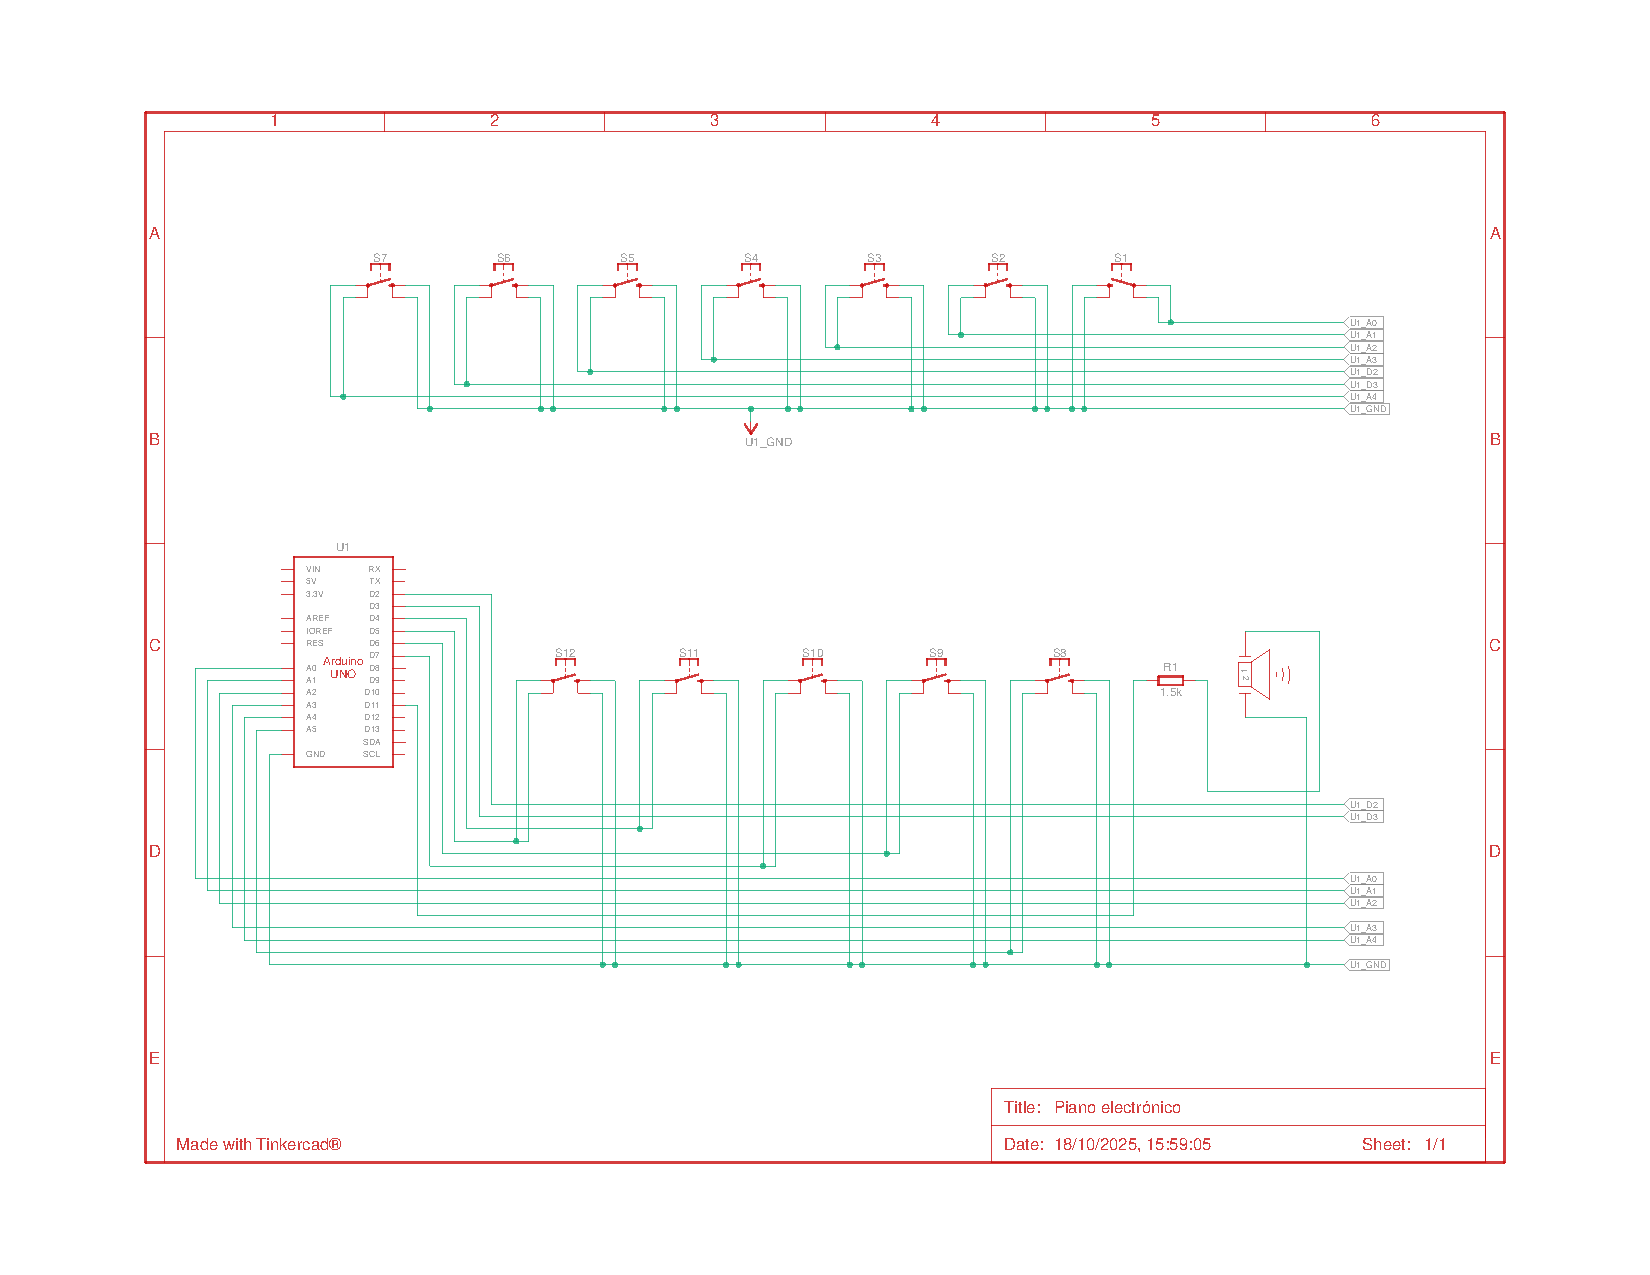
\includegraphics[width=0.5\textwidth]{Anexos/Conexionado_de_piano.pdf}
    \caption{Esquema de conexión del piano electrónico. Elavoración propia en Tinkercad®.}
    \label{fig:conexion_piano}
\end{figure}

\subsubsection{Cerradura electrónica}

En la Figura~\ref{fig:Cerradura_electronica} se presenta el esquema de conexión del sistema de cerradura electrónica. 
El circuito fue diseñado en Tinkercad® y muestra la interconexión entre el microcontrolador ATmega328P, el teclado matricial 4×4, 
la pantalla LCD 16×2 con interfaz I²C, los LEDs indicadores (rojo y verde) y el buzzer de señalización.

\begin{figure}[H]
    \centering
    \includegraphics[width=0.5\textwidth]{Anexos/Cerradura_electrónica.pdf}
    \caption{Esquema de conexión del candado electrónico. Elaboración propia en Tinkercad®.}
    \label{fig:Cerradura_electronica}
\end{figure}

\subsection{Códigos fuente}

\subsubsection{Piano electrónico}
A continuación se detalla la estructura de archivos del proyecto del piano electrónico:

\begin{verbatim}
-- main.c
-- piano.h
-- piano.c
-- sonidos.h
-- sonidos.c
-- funciones.h
-- funciones.c
-- figuras.h
-- figuras.c
-- canciones.h
-- canciones.c
-- hw_pins.h
-- hw_pins.c
-- uart.h
-- uart.c

\end{verbatim}

El código fuente completo del proyecto se encuentra disponible en el repositorio de GitHub \cite{utec_tecmicro}.

\subsection{Evidencias}
Las evidencias de la realización de los ejercicios del laboratorio dos, se encuentran adjuntas en la carpeta \textit{“Evidencias”} \cite{github_evidencias_lab2}. Dentro de ella, se encuentran las fotos, videos, documentos, que demuestran la correcta implementación y funcionamiento de los sistemas desarrollados en este laboratorio.

\subsection{Tablas complementarias}
\subsubsection{Correspondencia entre notas y frecuencias del piano electrónico}

En la Tabla~\ref{tab:notas_piano} se presenta la correspondencia entre las notas musicales, 
sus frecuencias y el índice utilizado dentro del arreglo \texttt{notas[]} en el programa del piano electrónico. 
Los valores corresponden a la octava número 4, considerada la octava base del sistema. 

\begin{table}[H]
\centering
\begin{tabular}{|c|c|c|c|}
\hline
\textbf{Nota} & \textbf{Frecuencia (Hz)} & \textbf{Índice en arreglo} & \textbf{Octava} \\
\hline
DO  & 262 & 0  & 4 \\
DO\# & 277 & 1  & 4 \\
RE  & 294 & 2  & 4 \\
RE\# & 311 & 3  & 4 \\
MI  & 330 & 4  & 4 \\
FA  & 349 & 5  & 4 \\
FA\# & 370 & 6  & 4 \\
SOL & 392 & 7  & 4 \\
SOL\# & 415 & 8  & 4 \\
LA  & 440 & 9  & 4 \\
LA\# & 466 & 10 & 4 \\
SI  & 494 & 11 & 4 \\
\hline
\end{tabular}
\caption{Correspondencia entre notas, frecuencias e índices de la octava 4 utilizada en el piano electrónico.}
\label{tab:notas_piano}
\end{table}

Las frecuencias de las octavas superiores (5, 6 y 7) se obtuvieron a partir de las frecuencias de referencia de la octava 4, 
utilizando la relación:

\[
f_{n} = f_{0} \times 2^{n}
\]

donde \( f_{n} \) representa la frecuencia de una nota en la octava \( n \), 
y \( f_{0} \) es la frecuencia de la misma nota en la octava base. 
De esta forma, el sistema puede reproducir diferentes rangos tonales de manera programática.

\subsubsection{Mapa de pines del piano electrónico}

En la Tabla~\ref{tab:pines_piano} se detalla la asignación de pines del microcontrolador ATmega328P utilizados en el proyecto del piano electrónico, incluyendo las funciones específicas de cada pin.

\begin{table}[H]
\centering
\resizebox{\columnwidth}{!}{%
\begin{tabular}{|c|c|c|}
\hline
\textbf{Señal} & \textbf{Pin Arduino} & \textbf{Descripción} \\
\hline
BUZZER (PWM) & D3 (OC2B) & Salida PWM para tono (Timer2). \\
UART\_TX     & D1 (TX)    & Transmisión serie a 9600 baud. \\
UART\_RX     & D0 (RX)    & Recepción serie (comandos). \\
TECLA 1..12  & D2, D4..D9, A0..A3 & Entradas con resistencias pull-up internas. \\
\hline
\end{tabular}
}
\caption{Asignación de pines utilizada en el piano electrónico.}
\label{tab:pines_piano}
\end{table}

\subsubsection{Comandos UART implementados}

Los comandos UART disponibles para el control del piano electrónico se presentan en la Tabla~\ref{tab:uart_piano}. 

\begin{table}[H]
\centering
\resizebox{\columnwidth}{!}{%
\begin{tabular}{|c|c|c|}
\hline
\textbf{Comando} & \textbf{Acción} & \textbf{Observación} \\
\hline
\texttt{C1}    & Reproduce canción 1. & Melodía predefinida en \texttt{canciones.c}. \\
\texttt{C2}    & Reproduce canción 2. & Melodía predefinida en \texttt{canciones.c}. \\
\texttt{PIANO} & Modo manual. & Habilita lectura de teclas 1..12. \\
\hline
\end{tabular}
}
\caption{Comandos UART disponibles para el control del piano electrónico.}
\label{tab:uart_piano}
\end{table}

Estos comandos permiten al usuario seleccionar entre la reproducción automática de melodías predefinidas o el modo manual para tocar notas individuales mediante los pulsadores conectados al microcontrolador.

\vspace{0.5cm}

\subsubsection{Figuras musicales y duración}

En la Tabla~\ref{tab:figuras_piano} se muestra la relación de duraciones empleada para programar las melodías en el piano electrónico.

\begin{table}[H]
\centering
\begin{tabular}{|l|c|c|}
\hline
\textbf{Figura} & \textbf{Relación vs negra} & \textbf{Ejemplo (ms) si negra = 500 ms} \\
\hline
Redonda  & $\times 4$   & 2000 \\
Blanca   & $\times 2$   & 1000 \\
Negra    & $\times 1$   & 500 \\
Corchea  & $\times 1/2$ & 250 \\
Semicor. & $\times 1/4$ & 125 \\
Semisemi. & $\times 1/8$ & 62.5 \\
\hline
\end{tabular}
\caption{Relación de duraciones empleada para programar las melodías.}
\label{tab:figuras_piano}
\end{table}

Estas duraciones permiten definir el ritmo de las melodías reproducidas por el piano electrónico, facilitando la programación de diferentes estilos musicales.